\documentclass[11pt]{article}
\usepackage[textwidth=18.0cm, textheight=23.0cm, top=2.0cm]{geometry}
\usepackage{pst-all}
\usepackage{amssymb}
\usepackage{tikz}
\usepackage{underscore}\begin{document}
\pagestyle{empty}


ClassName: \underline{\textbf{Class_06.2bp-17}}
\par
BinSize: \underline{\textbf{300 × 300}}
\par
ReduceSize: \underline{\textbf{300 × 300}}
\par
TypeNum: \underline{\textbf{40}}
\par
Num: \underline{\textbf{40}}
\par
OutS: \underline{\textbf{180000}}
\par
InS: \underline{\textbf{125010}}
\par
Rate: \underline{\textbf{0.695}}
\par
UB: \underline{\textbf{2}}
\par
LB0: \underline{\textbf{2}}
\par
LB: \underline{\textbf{2}}
\par
LBWithCut: \underline{\textbf{2}}
\par
NodeCut: \underline{\textbf{0}}
\par
ExtendedNodeCnt: \underline{\textbf{1}}
\par
GenNodeCnt: \underline{\textbf{1}}
\par
PrimalNode: \underline{\textbf{0}}
\par
ColumnCount: \underline{\textbf{2}}
\par
TotalCutCount: \underline{\textbf{0}}
\par
RootCutCount: \underline{\textbf{0}}
\par
LPSolverCnt: \underline{\textbf{1}}
\par
PricingSolverCnt: \underline{\textbf{0}}
\par
BranchAndBoundNum: \underline{\textbf{1}}
\par
isOpt: \underline{\textbf{true}}
\par
TimeOnInitSolution: \underline{\textbf{600.000 s}}
\par
TimeOnPrimal: \underline{\textbf{0.000 s}}
\par
TimeOnPricing: \underline{\textbf{0.000 s}}
\par
TimeOnRmp: \underline{\textbf{0.070 s}}
\par
TotalTime: \underline{\textbf{600.375 s}}
\par
\newpage


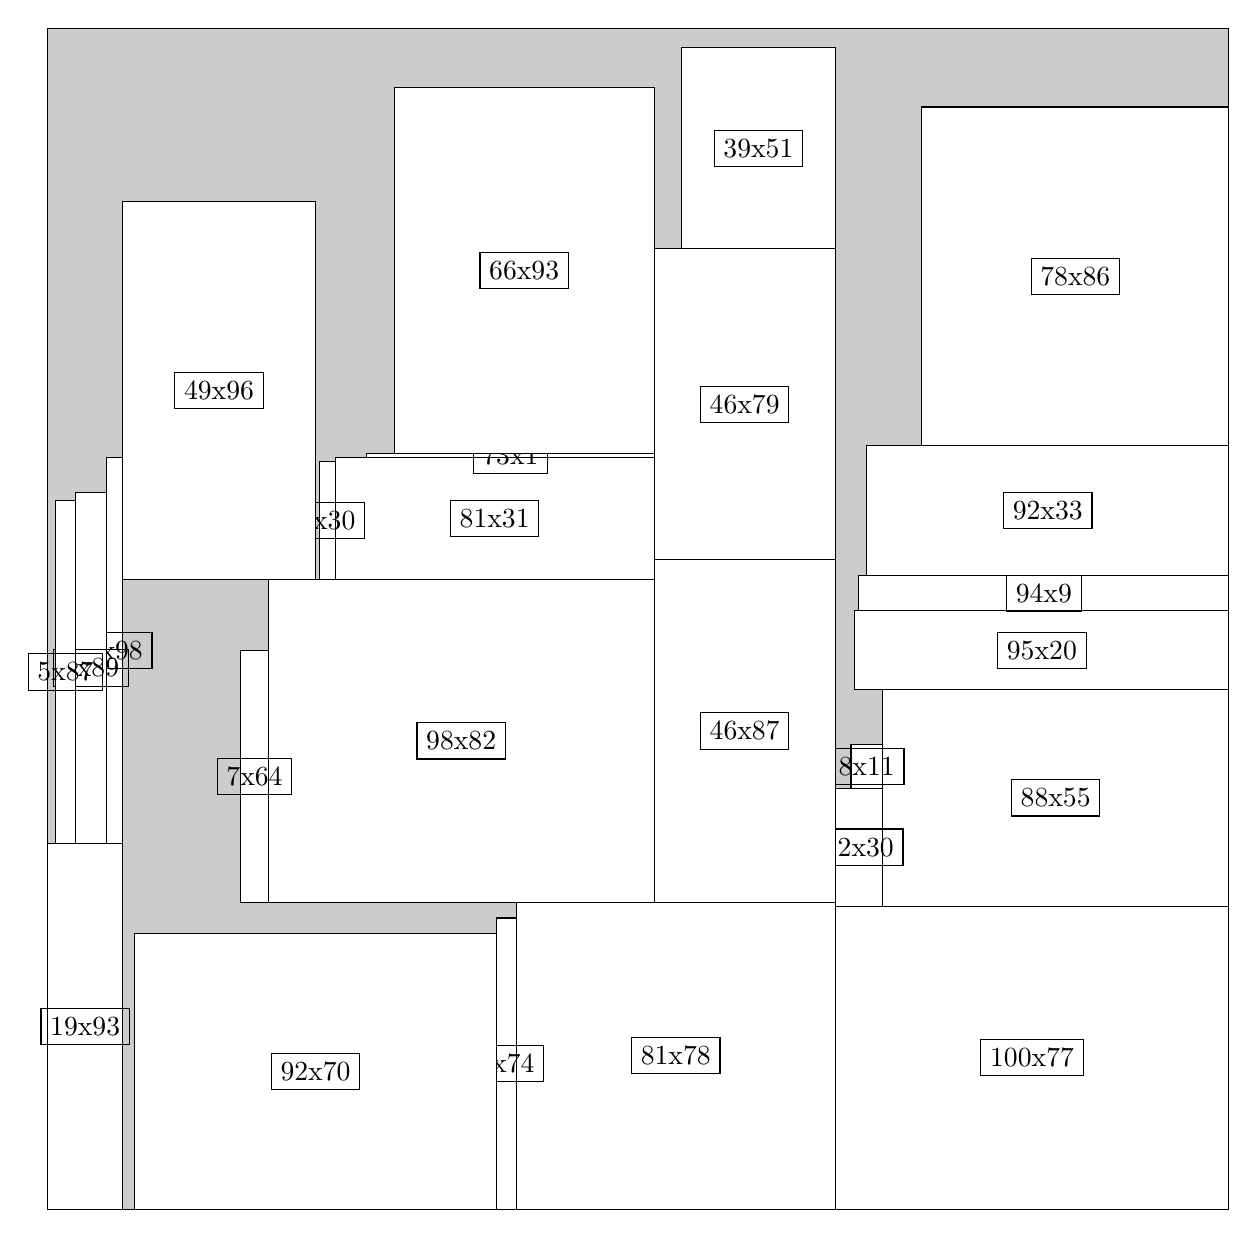
\begin{tikzpicture}[shorten >=1pt,scale=1.0,every node/.style={scale=1.0},->]
\tikzstyle{vertex}=[circle,fill=black!25,minimum size=14pt,inner sep=0pt]
\filldraw[fill=gray!40!white, draw=black] (0,0) rectangle (15.0,15.0);
\foreach \name/\x/\y/\w/\h in {100x77/10.0/0.0/5.0/3.85,88x55/10.600000000000001/3.85/4.4/2.75,12x30/10.0/3.85/0.6000000000000001/1.5,8x11/10.200000000000001/5.3500000000000005/0.4/0.55,95x20/10.25/6.6000000000000005/4.75/1.0,94x9/10.3/7.6000000000000005/4.7/0.45,92x33/10.4/8.05/4.6000000000000005/1.6500000000000001,78x86/11.100000000000001/9.700000000000001/3.9000000000000004/4.3,81x78/5.95/0.0/4.05/3.9000000000000004,5x74/5.7/0.0/0.25/3.7,92x70/1.1/0.0/4.6000000000000005/3.5,46x87/7.7/3.9000000000000004/2.3000000000000003/4.3500000000000005,46x79/7.7/8.25/2.3000000000000003/3.95,39x51/8.05/12.200000000000001/1.9500000000000002/2.5500000000000003,98x82/2.8000000000000003/3.9000000000000004/4.9/4.1000000000000005,7x64/2.45/3.9000000000000004/0.35000000000000003/3.2,81x31/3.6500000000000004/8.0/4.05/1.55,4x30/3.45/8.0/0.2/1.5,73x1/4.05/9.55/3.6500000000000004/0.05,66x93/4.4/9.600000000000001/3.3000000000000003/4.65,49x96/0.9500000000000001/8.0/2.45/4.800000000000001,19x93/0.0/0.0/0.9500000000000001/4.65,4x98/0.75/4.65/0.2/4.9,8x89/0.35000000000000003/4.65/0.4/4.45,5x87/0.1/4.65/0.25/4.3500000000000005}
\filldraw[fill=white!40!white, draw=black] (\x,\y) rectangle node[draw] (\name) {\name} ++(\w,\h);
\end{tikzpicture}


w =100 , h =77 , x =200 , y =0 , v =7700
\par
w =88 , h =55 , x =212 , y =77 , v =4840
\par
w =12 , h =30 , x =200 , y =77 , v =360
\par
w =8 , h =11 , x =204 , y =107 , v =88
\par
w =95 , h =20 , x =205 , y =132 , v =1900
\par
w =94 , h =9 , x =206 , y =152 , v =846
\par
w =92 , h =33 , x =208 , y =161 , v =3036
\par
w =78 , h =86 , x =222 , y =194 , v =6708
\par
w =81 , h =78 , x =119 , y =0 , v =6318
\par
w =5 , h =74 , x =114 , y =0 , v =370
\par
w =92 , h =70 , x =22 , y =0 , v =6440
\par
w =46 , h =87 , x =154 , y =78 , v =4002
\par
w =46 , h =79 , x =154 , y =165 , v =3634
\par
w =39 , h =51 , x =161 , y =244 , v =1989
\par
w =98 , h =82 , x =56 , y =78 , v =8036
\par
w =7 , h =64 , x =49 , y =78 , v =448
\par
w =81 , h =31 , x =73 , y =160 , v =2511
\par
w =4 , h =30 , x =69 , y =160 , v =120
\par
w =73 , h =1 , x =81 , y =191 , v =73
\par
w =66 , h =93 , x =88 , y =192 , v =6138
\par
w =49 , h =96 , x =19 , y =160 , v =4704
\par
w =19 , h =93 , x =0 , y =0 , v =1767
\par
w =4 , h =98 , x =15 , y =93 , v =392
\par
w =8 , h =89 , x =7 , y =93 , v =712
\par
w =5 , h =87 , x =2 , y =93 , v =435
\par
\newpage


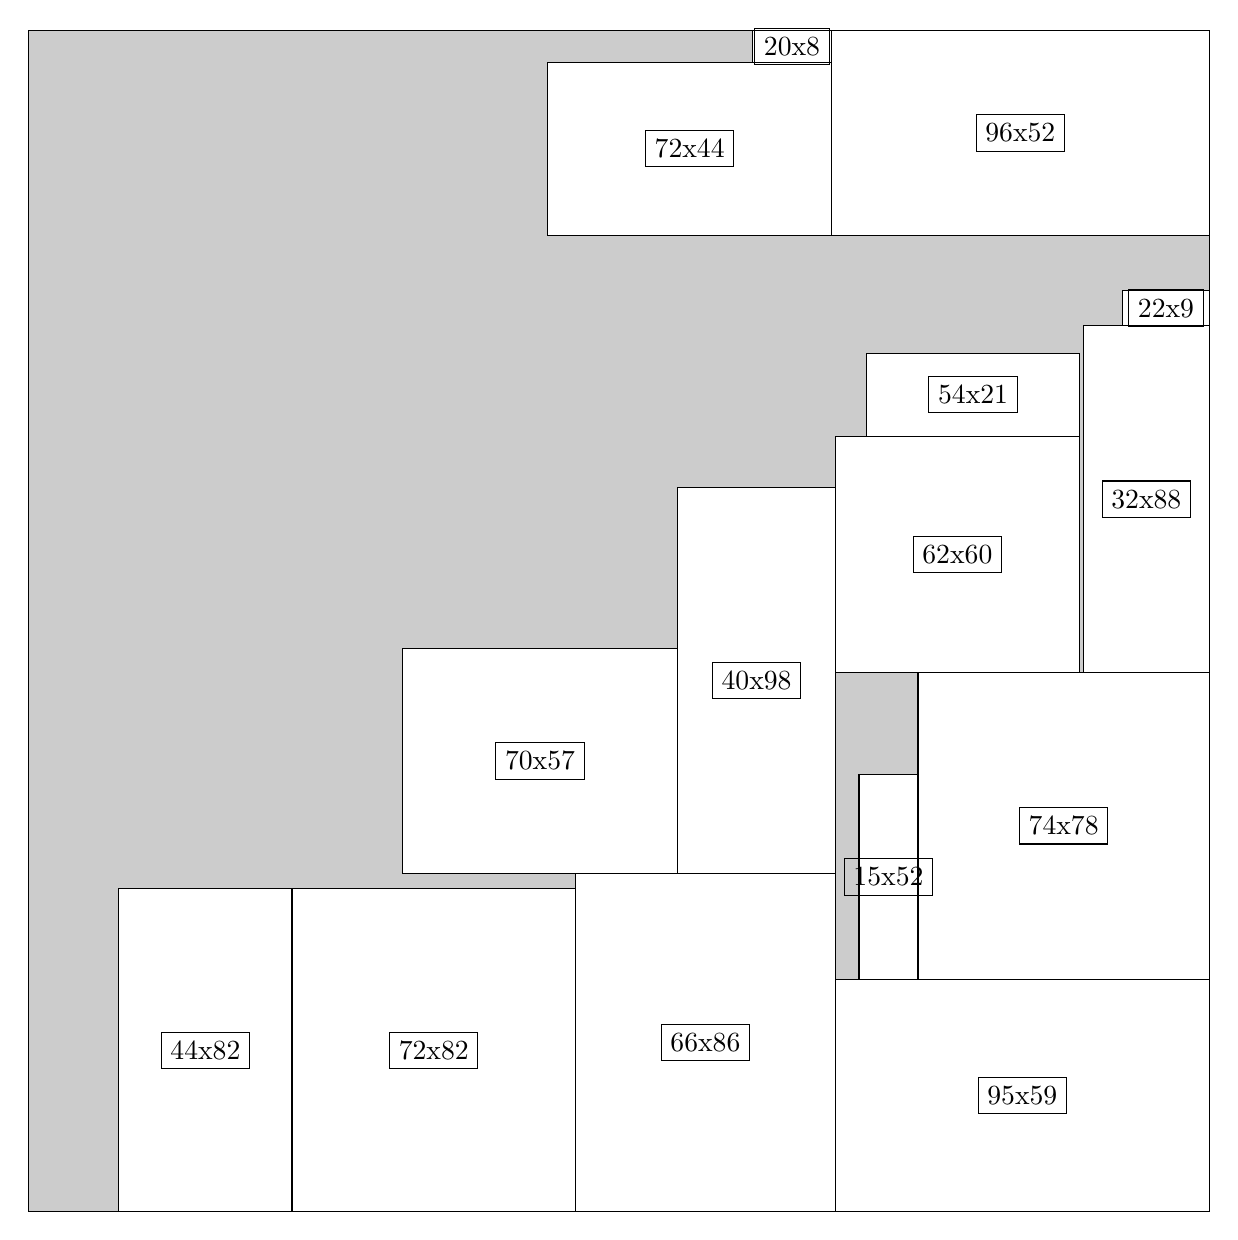
\begin{tikzpicture}[shorten >=1pt,scale=1.0,every node/.style={scale=1.0},->]
\tikzstyle{vertex}=[circle,fill=black!25,minimum size=14pt,inner sep=0pt]
\filldraw[fill=gray!40!white, draw=black] (0,0) rectangle (15.0,15.0);
\foreach \name/\x/\y/\w/\h in {95x59/10.25/0.0/4.75/2.95,74x78/11.3/2.95/3.7/3.9000000000000004,15x52/10.55/2.95/0.75/2.6,32x88/13.4/6.8500000000000005/1.6/4.4,22x9/13.9/11.25/1.1/0.45,62x60/10.25/6.8500000000000005/3.1/3.0,54x21/10.65/9.850000000000001/2.7/1.05,66x86/6.95/0.0/3.3000000000000003/4.3,72x82/3.35/0.0/3.6/4.1000000000000005,44x82/1.1500000000000001/0.0/2.2/4.1000000000000005,40x98/8.25/4.3/2.0/4.9,70x57/4.75/4.3/3.5/2.85,96x52/10.200000000000001/12.4/4.800000000000001/2.6,72x44/6.6000000000000005/12.4/3.6/2.2,20x8/9.200000000000001/14.600000000000001/1.0/0.4}
\filldraw[fill=white!40!white, draw=black] (\x,\y) rectangle node[draw] (\name) {\name} ++(\w,\h);
\end{tikzpicture}


w =95 , h =59 , x =205 , y =0 , v =5605
\par
w =74 , h =78 , x =226 , y =59 , v =5772
\par
w =15 , h =52 , x =211 , y =59 , v =780
\par
w =32 , h =88 , x =268 , y =137 , v =2816
\par
w =22 , h =9 , x =278 , y =225 , v =198
\par
w =62 , h =60 , x =205 , y =137 , v =3720
\par
w =54 , h =21 , x =213 , y =197 , v =1134
\par
w =66 , h =86 , x =139 , y =0 , v =5676
\par
w =72 , h =82 , x =67 , y =0 , v =5904
\par
w =44 , h =82 , x =23 , y =0 , v =3608
\par
w =40 , h =98 , x =165 , y =86 , v =3920
\par
w =70 , h =57 , x =95 , y =86 , v =3990
\par
w =96 , h =52 , x =204 , y =248 , v =4992
\par
w =72 , h =44 , x =132 , y =248 , v =3168
\par
w =20 , h =8 , x =184 , y =292 , v =160
\par
\newpage


\end{document}